
In this section we will consider Statement 1, interpreting the effective Lorentz factor as the expectation value
of a particle's Lorentz factor.

In order to test this formulation we carried our the following simulation: we injected three 10-particle
bunches (X, Y, and D) into the ideal FS lattice. The orbital and spin transfer maps were computed
up to the third-order Taylor expansion; the particle injection energy was 270~MeV. The X-bunch particles
were uniformly distributed along the radial axis in the range $\pm 1$ mm; those of the Y-bunch, along the vertical
axis in the range $\pm 1.318$ mm;~\footnote{This range was chosen in order to equalize the transverse
emittances of the particles. The initial coordinate offset determines the betatron oscillation amplitude $A$,
which is related to the beta function $\beta$ and transverse emittance $\epsilon$ as in
$A = \sqrt{\epsilon \beta}$.} the D-bunch particles were distributed by $\Delta K/K_0$ in the range $\pm 10^{-4}$.
Then, spin tracking was done for 12,000 turns, with data recorded every 80 turns.

The recorded data were: 
\begin{enumerate}[(i)]
	\item the particle phase space coordinate $\vec z~=~(x,x',y,y',\ell, \delta)$, where
$\ell~=~-(t-t_0)v_0\frac{\gamma_0}{1+\gamma_0}$ is its longitudinal phase offset, 
$\delta~=~\Delta K/K$ is the energy offset;
\item spin tune $\nu_s(\vec z)$.
\end{enumerate}
Based on these data we computed the particles' time-average spin tune $\avg{\nu_s}$,
energy offset  $\avg{\Delta K/K}$, and longitudinal and transverse emittances.

Simulation results are presented in Figure~\ref{fig:stune_traj_equ_main}. The top panel is a plot of $\avg{\nu_s}$ as a function of $\avg{\Delta K/K}$ for the betatron-oscillating bunches when the sextupoles
are turned off. One can see from the figure that, at the same mean energy level, the horizontal plane
 betatron oscillating particles have a different spin tune from that of the vertical plane betatron
oscillating particles. This means, as far as we can tell, that Statement 1 in formulation A is disproved.

We hypothesized that the difference in the plotted lines' slopes is related to the
\emph{spatial dependence} of the momentum compaction factor.

This hypothesis is based on our analysis of the sextupole field suppression effects' signatures, described
in detail in section~\ref{sec:sext_decoh_suppression_effect_analysis}. In order to test this hypothesis we
repeated the experiment at different values of the GSX sextupole gradient, taken from
the range $\pm 5\cdot 10^{-3}$. The simulation results are shown in Figure~\ref{fig:stune_traj_equ_main}.
The same dependence is plotted as previously, but only for the X-bunch.
As one can see, when the gradient is varied the slope varies with it. The same behavior as was
observed in section~\ref{sec:sext_decoh_suppression_effect_analysis}.

\begin{figure}[h]
	\centering
	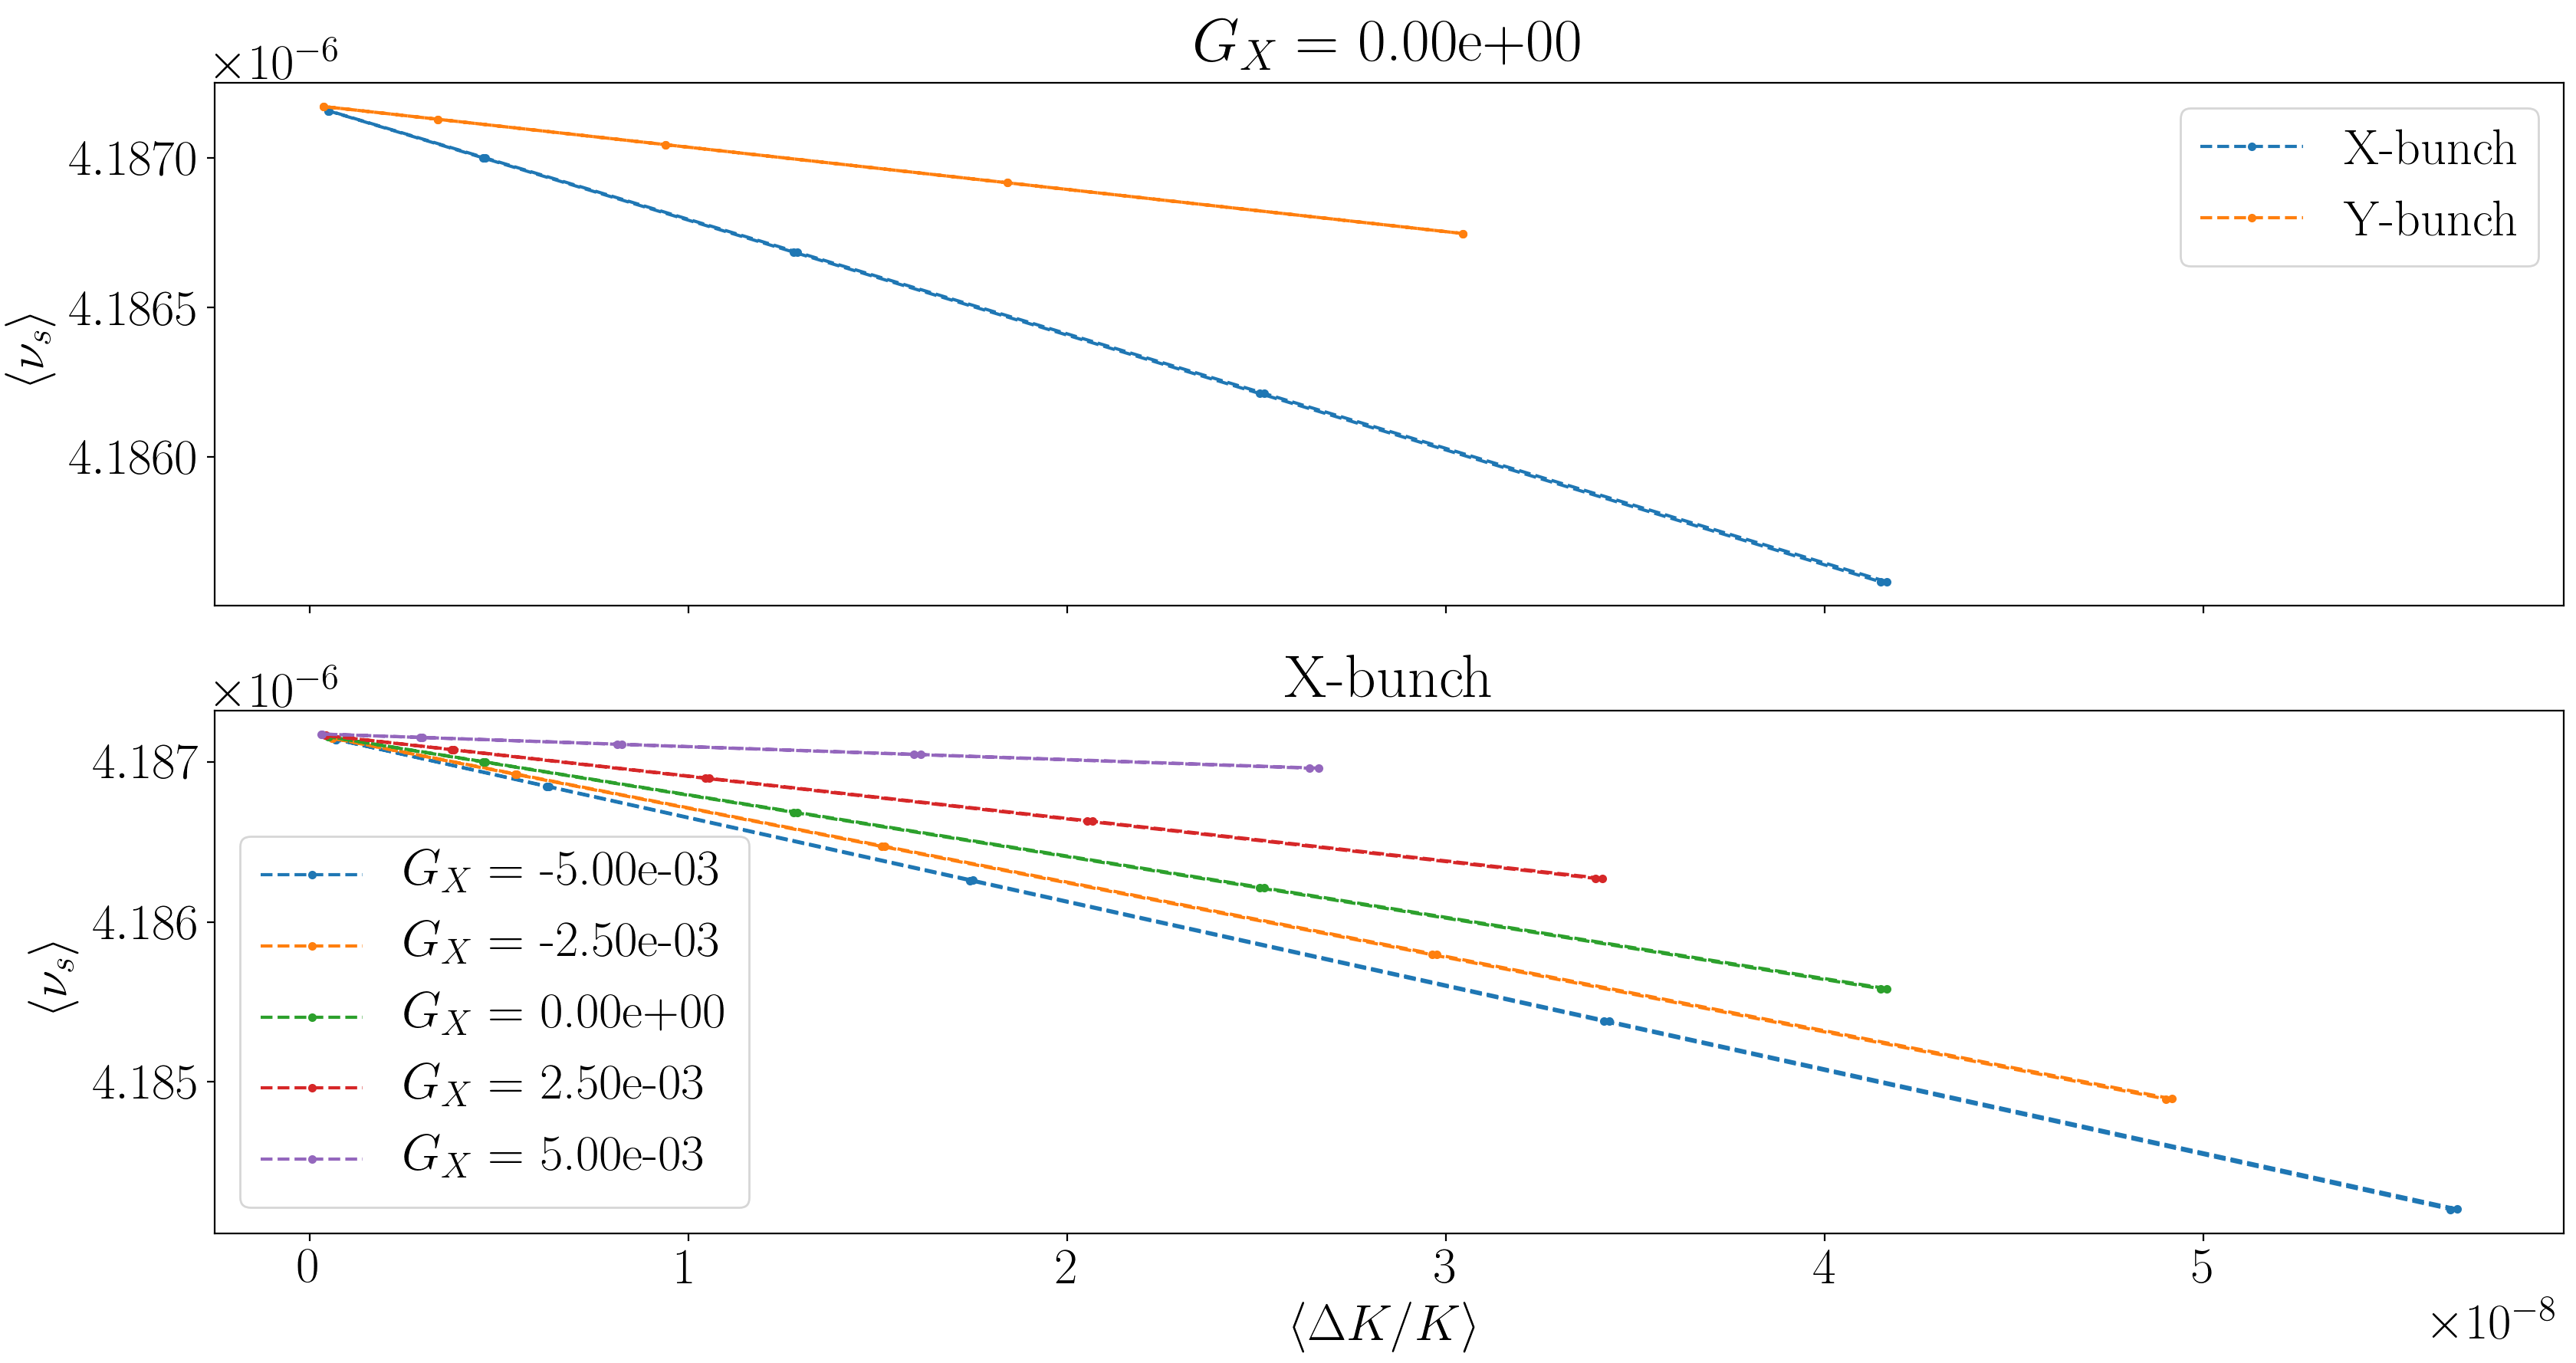
\includegraphics[height=.3\paperheight]{images/stune_traj_equ/part1/stune_vs_equ_energy}
	\caption[Mean spin tune level veresus mean kinetic energy level.]{Particle mean spin tune level
        as a function of its mean kinetic energy level. Top panel: sextupoles are off for both injected bunches.
        Bottom panel: X-bunch dependencies at different GSX gradients.\label{fig:stune_traj_equ_main}}
\end{figure}

In order to check the hypothesis about the spatial dependence of the momentum compaction factor we computed
the dependencies of the mean energy levels of the X- and Y-bunch particles on their betatron tune-normalized
transverse emittances (Fiugre~\ref{fig:equ_nrg_vs_emittance}).
According to equation~\eqref{eq:betatron_OL}, the orbit lengthening of particles with equal Q-normalized
transverse emittances must be equal. The equilibrium energy level shift of a particle is proportional to
its orbit lengthening via the momentum compaction factor; hence the slope difference seen in
Figure~\ref{fig:equ_nrg_vs_emittance} is evidence that the momentum compaction factors experienced by the
X-, and Y-bunches are different. 

\begin{figure}[h]
	\centering
	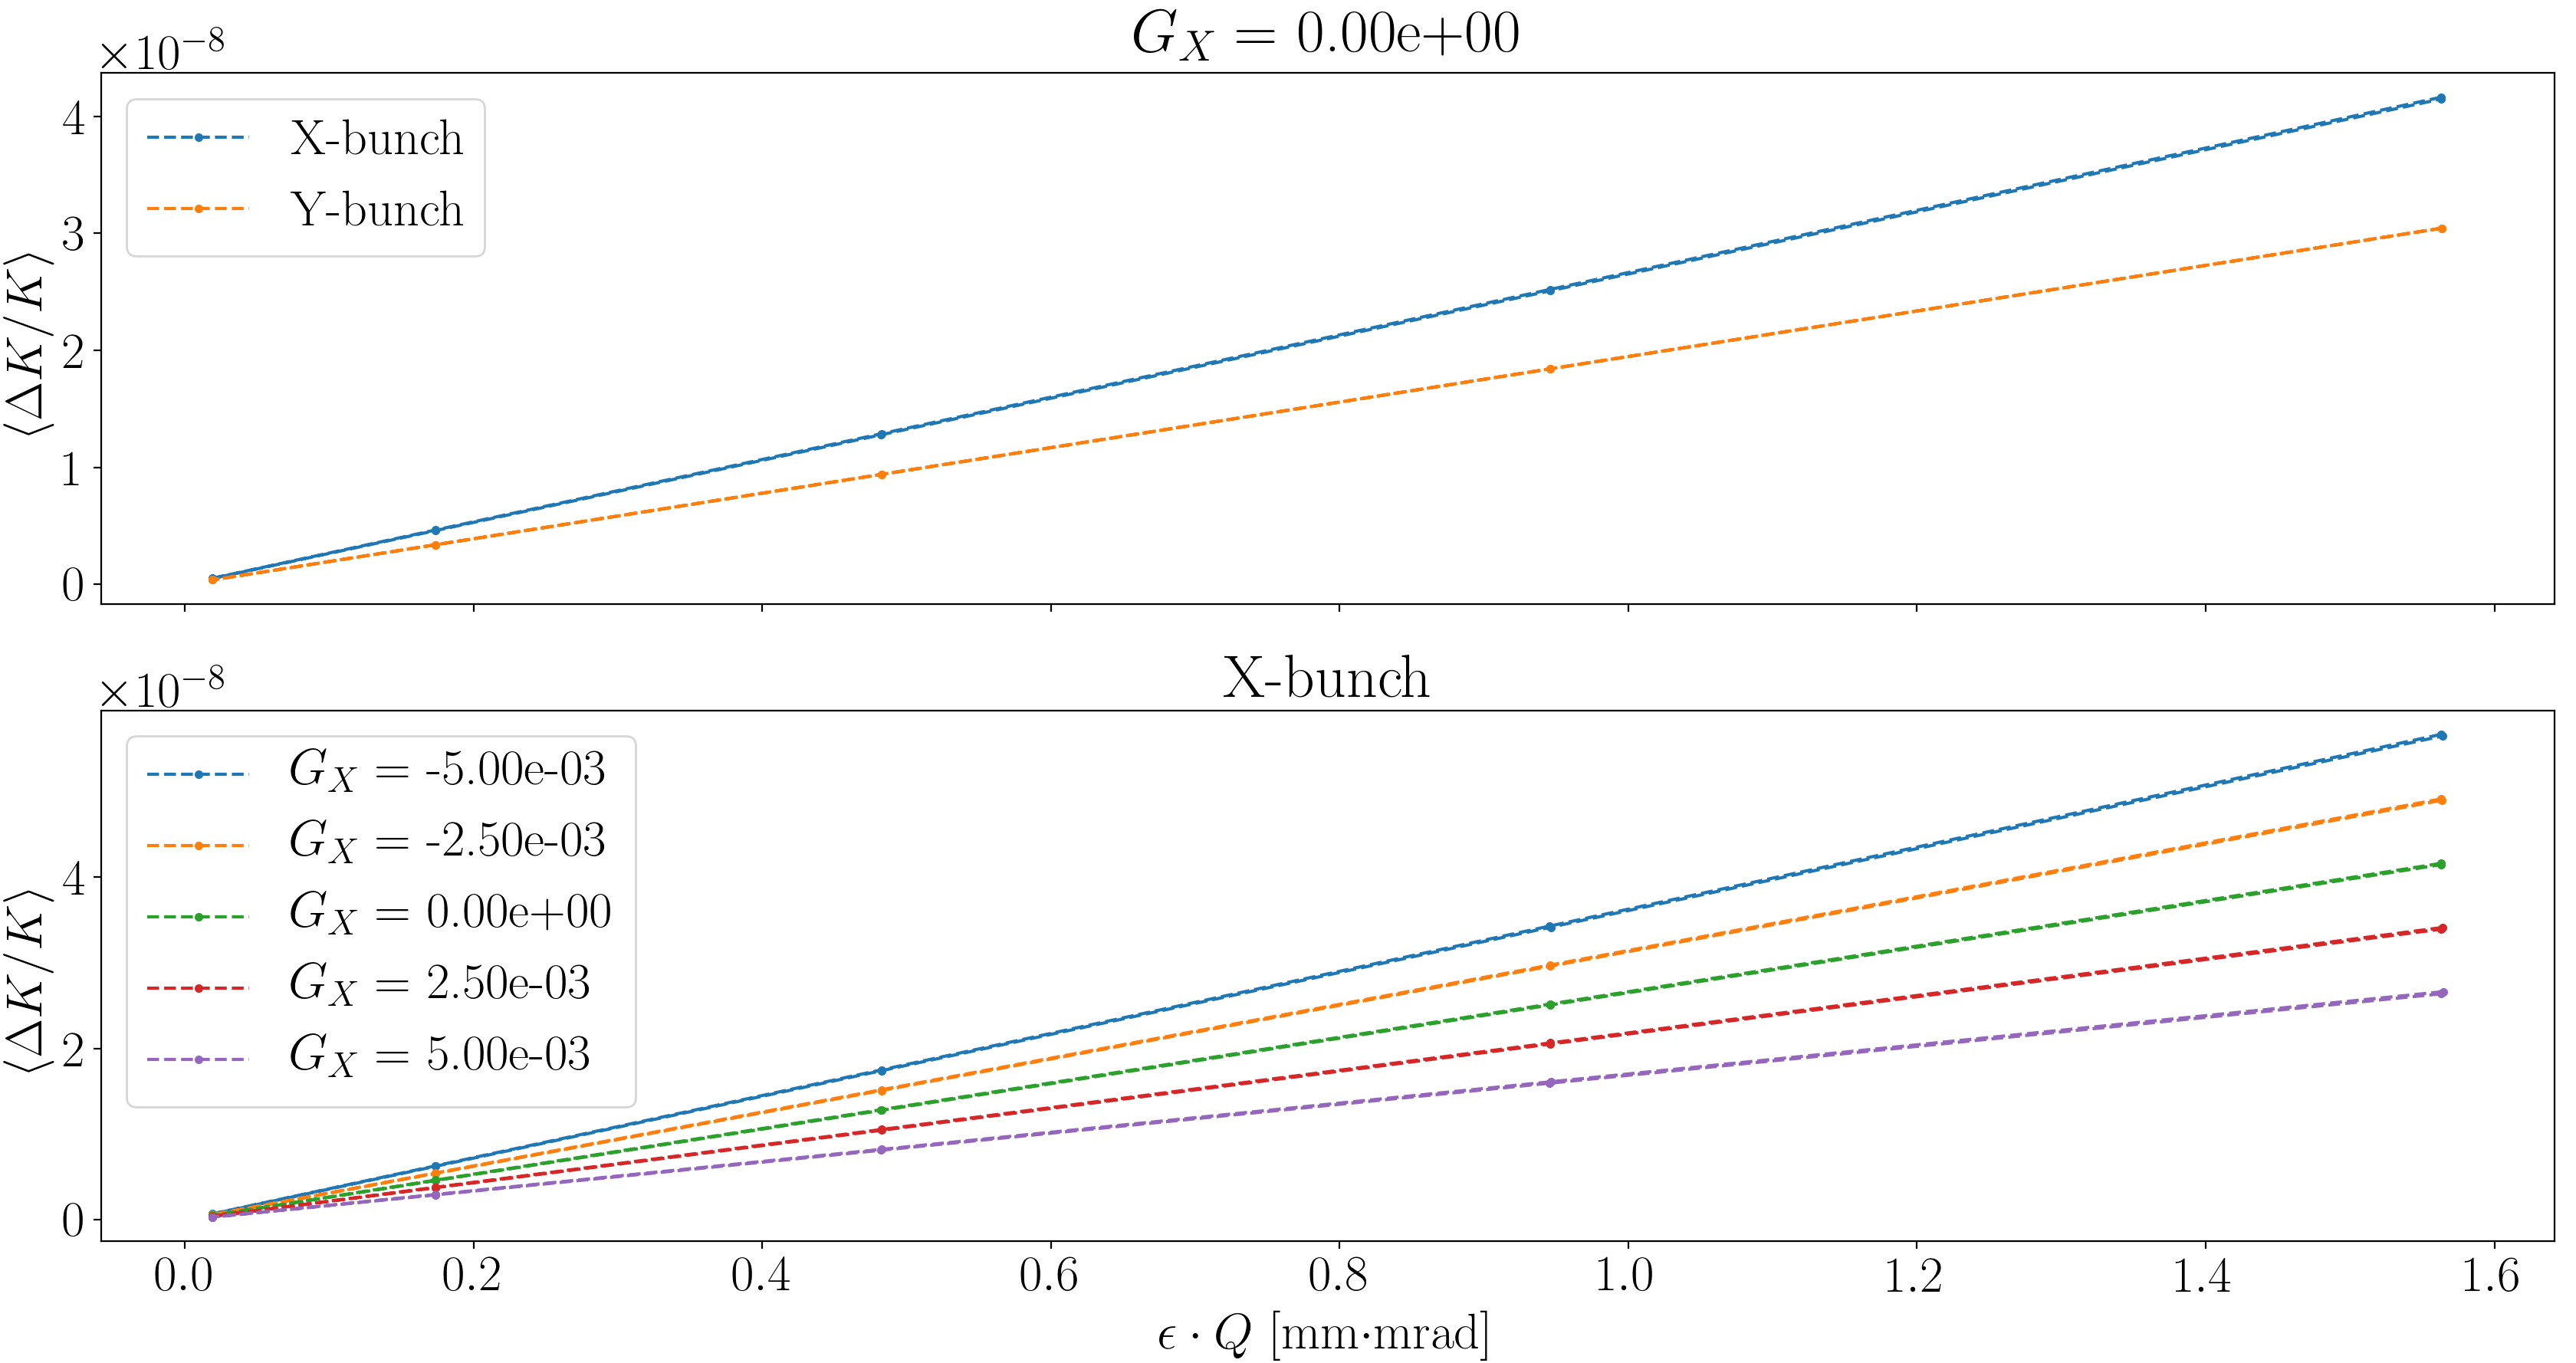
\includegraphics[height=.3\paperheight]{images/stune_traj_equ/part1/equ_energy_vs_emittance}
	\caption{Longitudinal emittance dependence of the mean energy level.\label{fig:equ_nrg_vs_emittance}}
\end{figure}

The observed longitudinal dependence of the momentum compaction factor is further confirmed by equation~(15)
of reference~\cite{Senichev:IPAC13}, in which we find:
\[
\alpha_0 = \avg{\frac{D_0}{\rho}},~~ \alpha_1 = \avg{\frac{D_1}{\rho}} + \frac12\avg{D_0'^2},
\]
where $D(s) = D_0(s) + D_1(s)\cdot \delta$  is the dispersion function, $\rho$ the radius of the clsed orbit.
In first approximation, dispersion exists only in the horizontal plane and is zero in the vertical plane,
meaning that the spatial dependence of the dispersion function reflects on the spatial dependence of the momentum
compaction factor.

For comparison, the same tests were carried out with linear Taylor expansions of the spin and orbital
transfer maps. The results are shown in Figures~\ref{fig:stune_traj_equ_linear:stune_vs_nrg},
and~\ref{fig:stune_traj_equ_linear:nrg_vs_emittance}. As one can see in
Figure~\ref{fig:stune_traj_equ_linear:nrg_vs_emittance}, all particles doing betatron oscillations in the
vertical plane share the same value of the mean energy level, which is an indication that they share
the same closed orbit, which in turn means there's no dispersion in the vertical plane.
In this case, from Figure~\ref{fig:stune_traj_equ_linear:stune_vs_nrg} follows that their spin tunes
are equal.

\begin{figure}[h]
\centering
\begin{subfigure}{\linewidth}
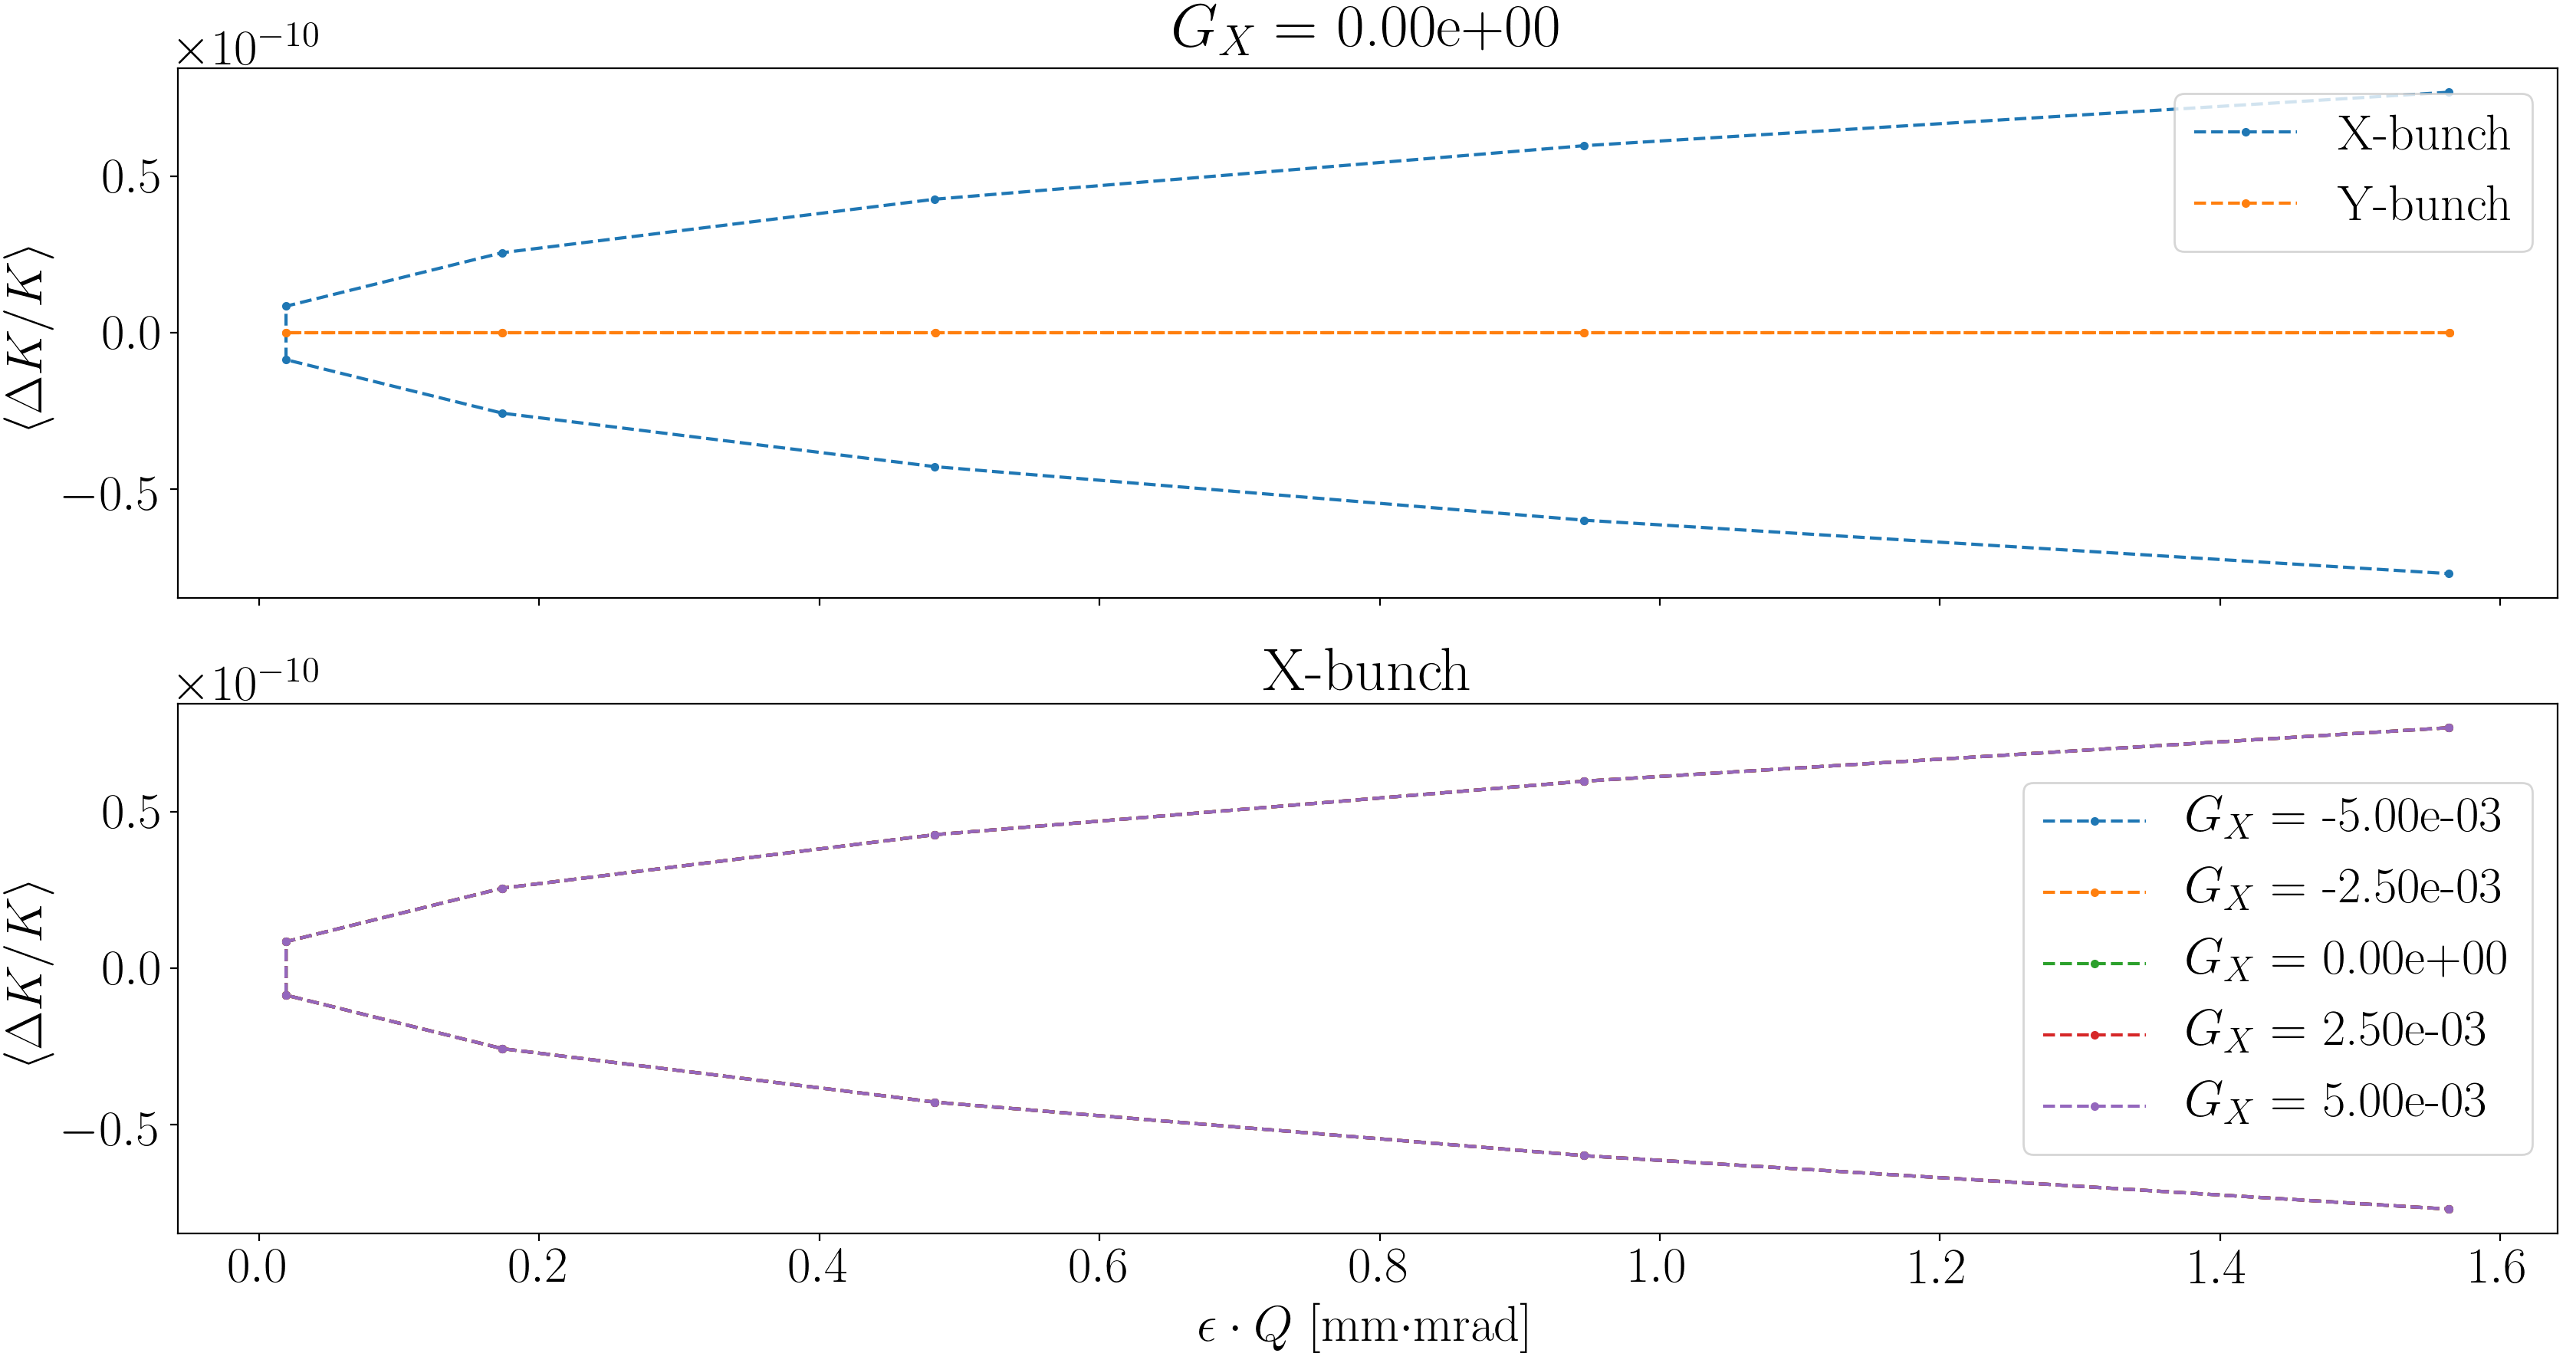
\includegraphics[width=\linewidth]{images/stune_traj_equ/part1/equ_energy_vs_emittance_linear}
\caption{Mean energy level dependence on
particle transverse emittance\label{fig:stune_traj_equ_linear:nrg_vs_emittance}}
\end{subfigure} 
\begin{subfigure}{\linewidth}
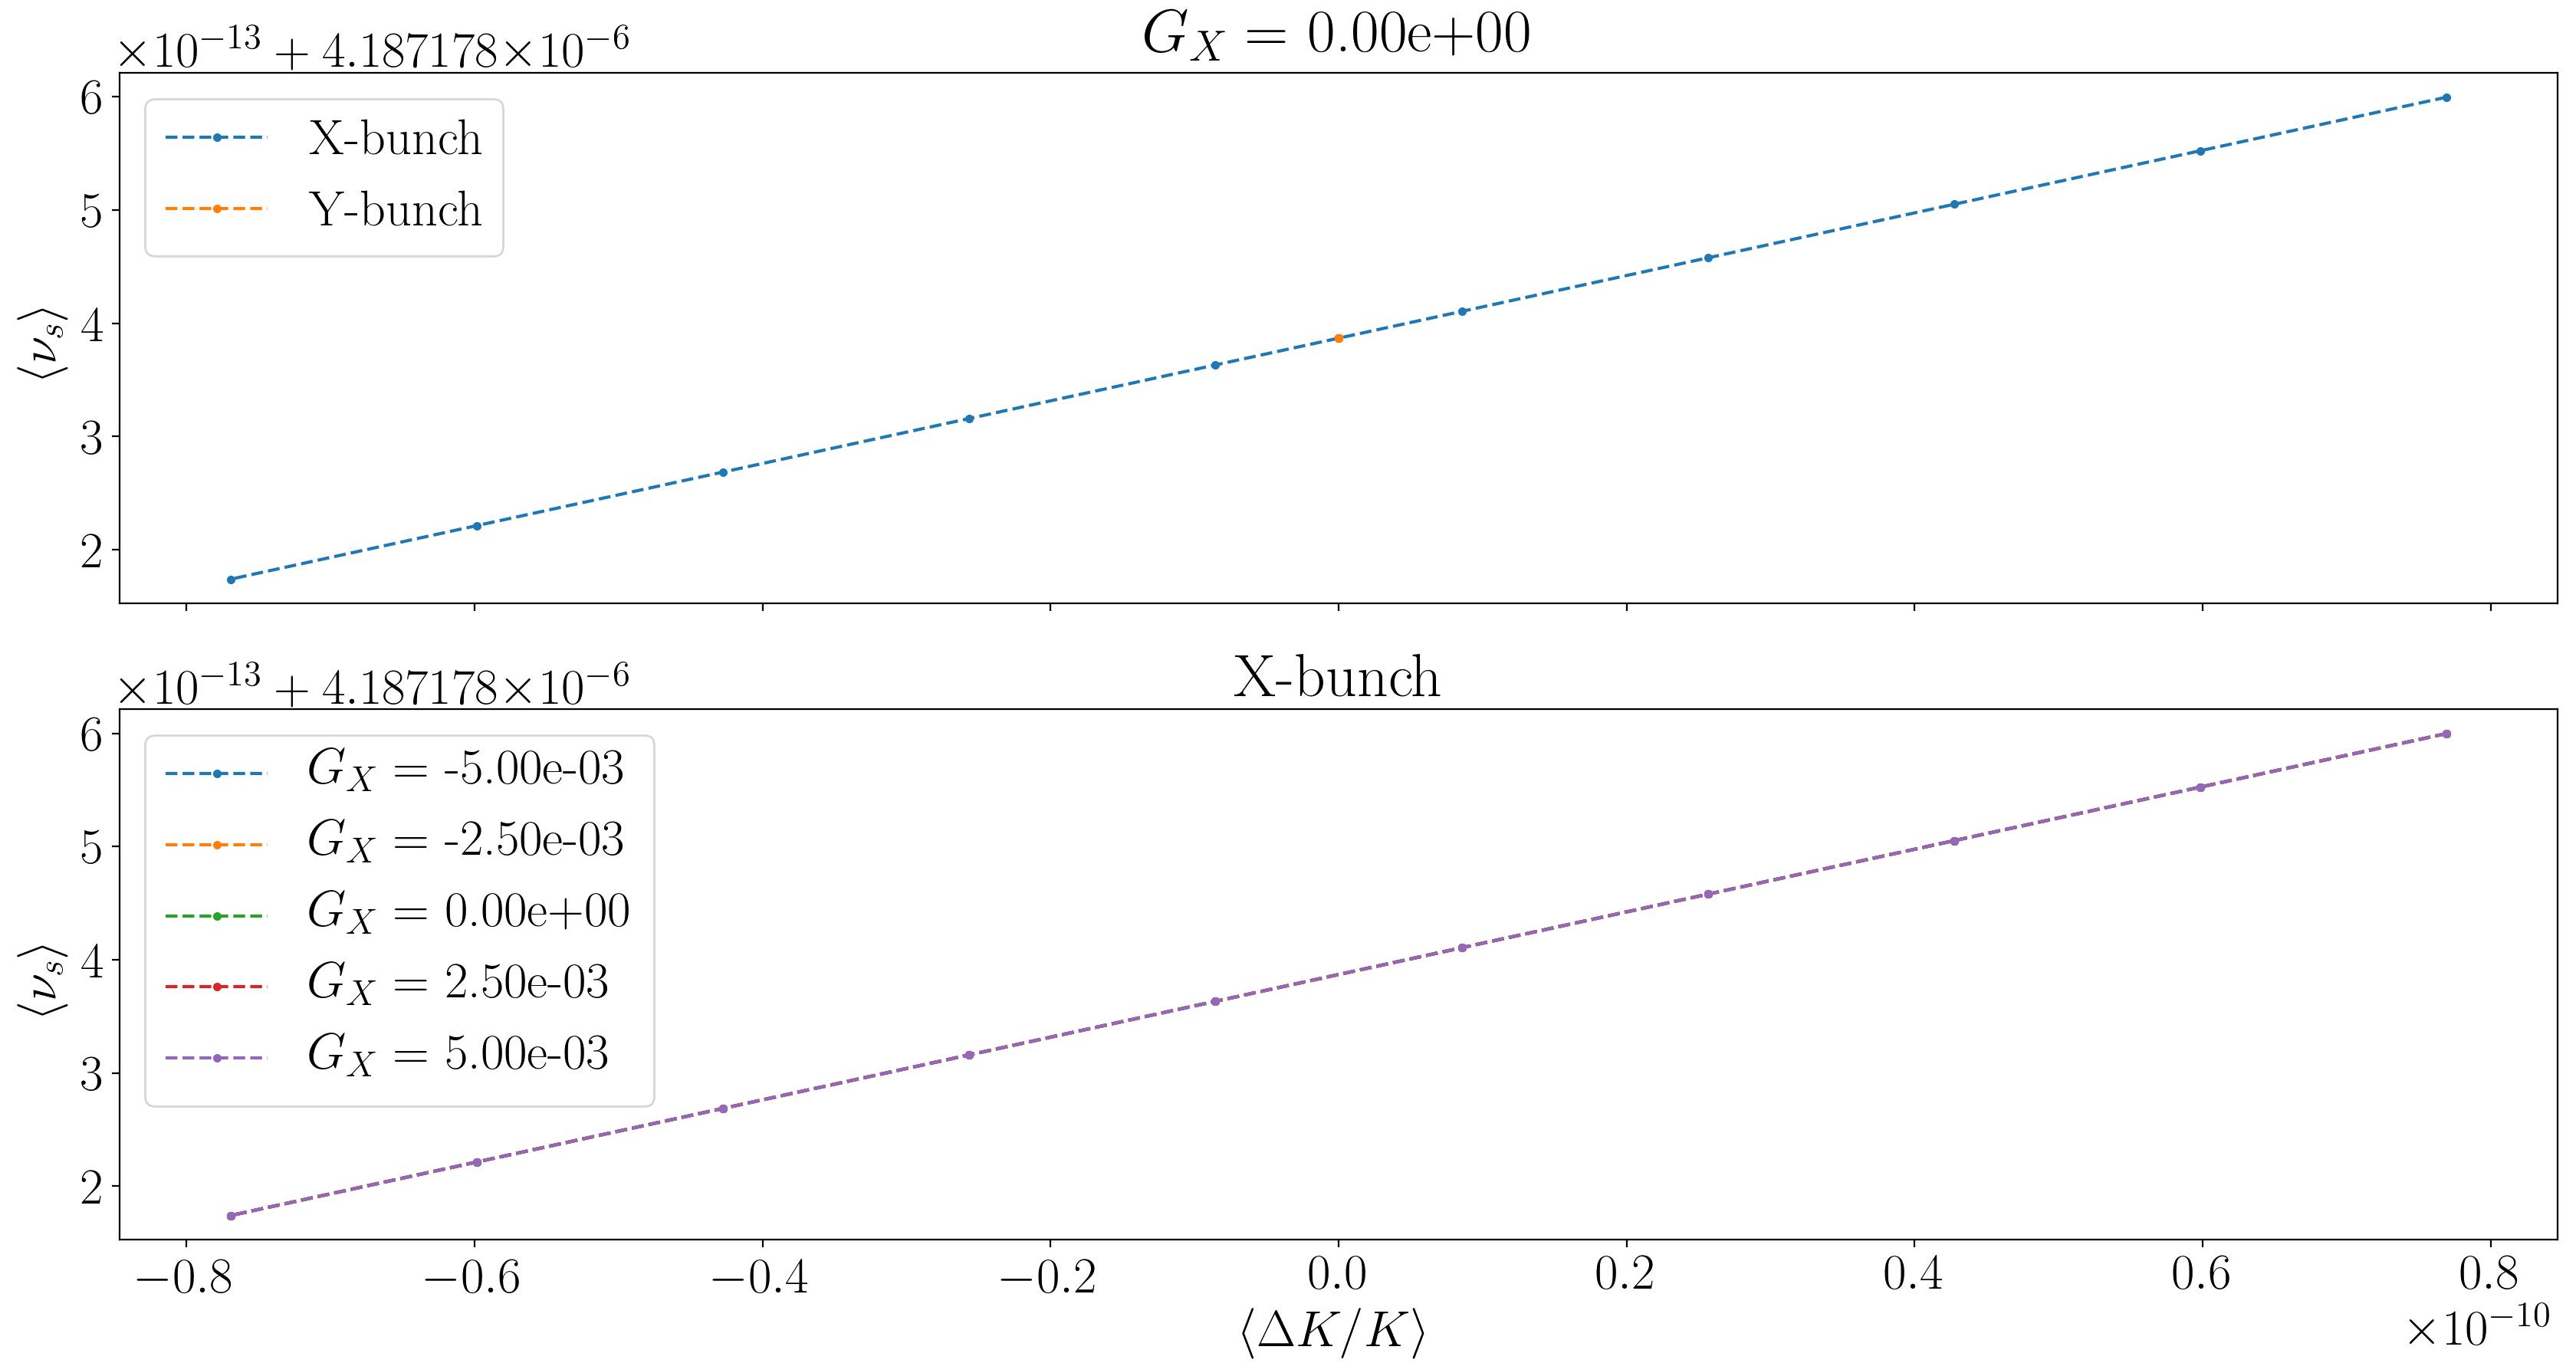
\includegraphics[width=\linewidth]{images/stune_traj_equ/part1/stune_vs_equ_energy_linear}
\caption{Mean spin tune dependence on mean energy.\label{fig:stune_traj_equ_linear:stune_vs_nrg}}
\end{subfigure} 
\caption{Simulation results in the case of linear transfer maps.}
\end{figure}

In Figure~\ref{fig:long_emitt_vs_trans_emitt} are plotted the particle longitudinal emittance as a
function of its Q-normalized transverse emittance. As one can see, the transverse emittances induce
the longitudianl emittances at different rates, depending on the betatron oscillation plane.
In the linear case, vertical plane betatron oscillations do not induce synchrotron oscillations at all.
\begin{figure}[h]
\centering
\begin{subfigure}{\linewidth}
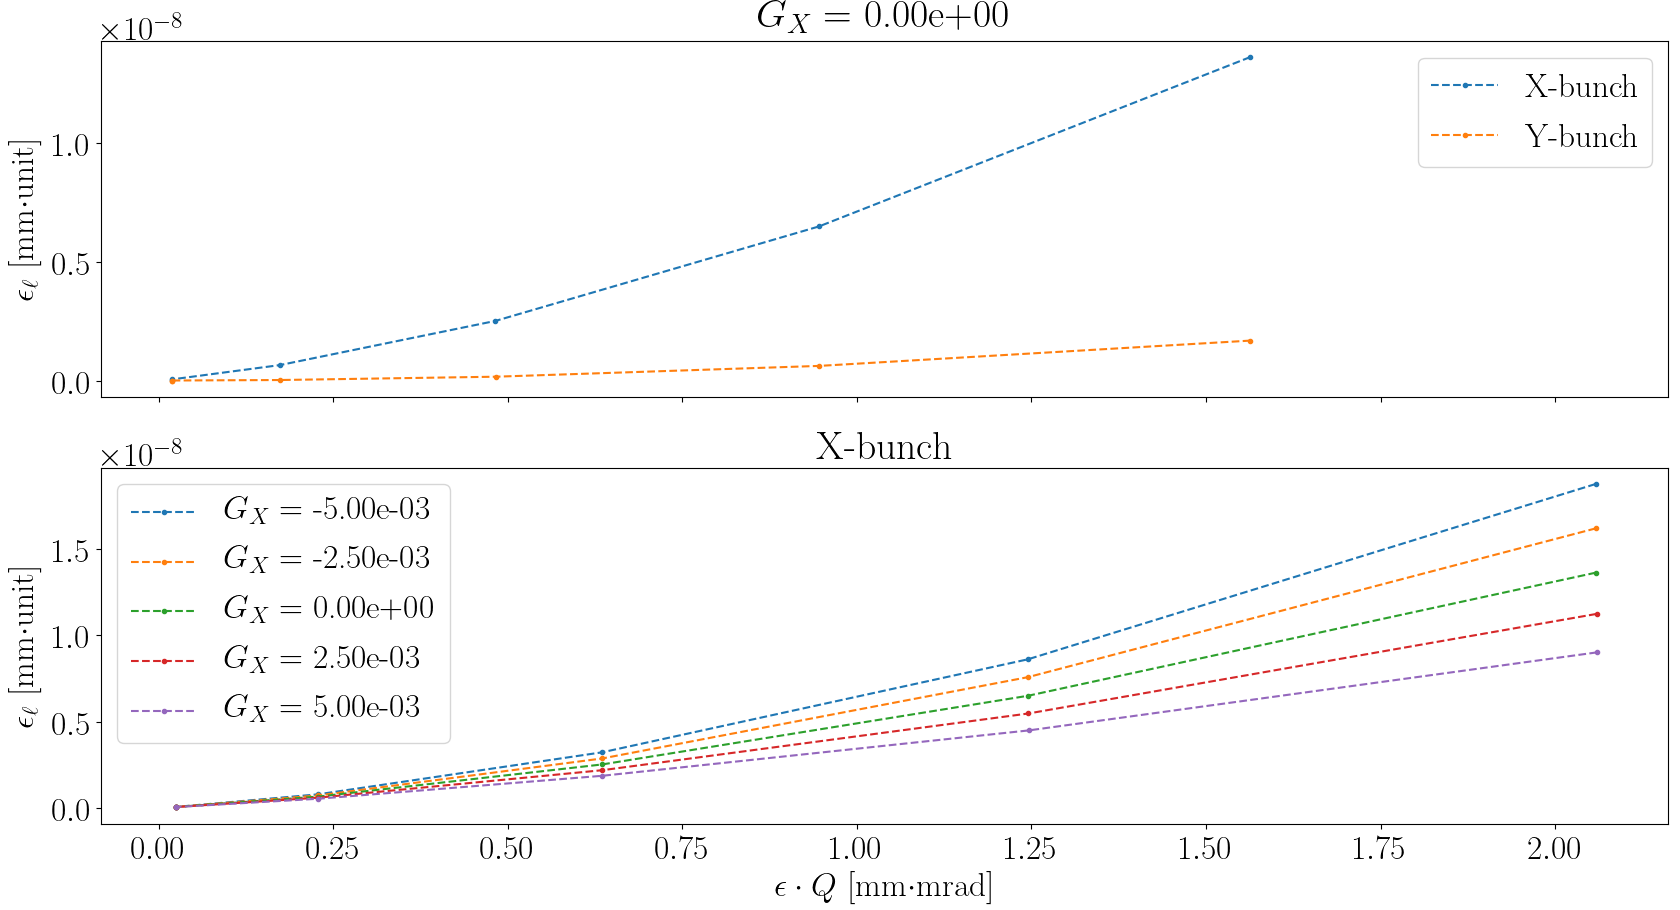
\includegraphics[height=.3\paperheight]{images/stune_traj_equ/part1/long_emitt_vs_trans_emitt}
\caption{Non-linear transfer maps.}
\end{subfigure}
\begin{subfigure}{\linewidth}
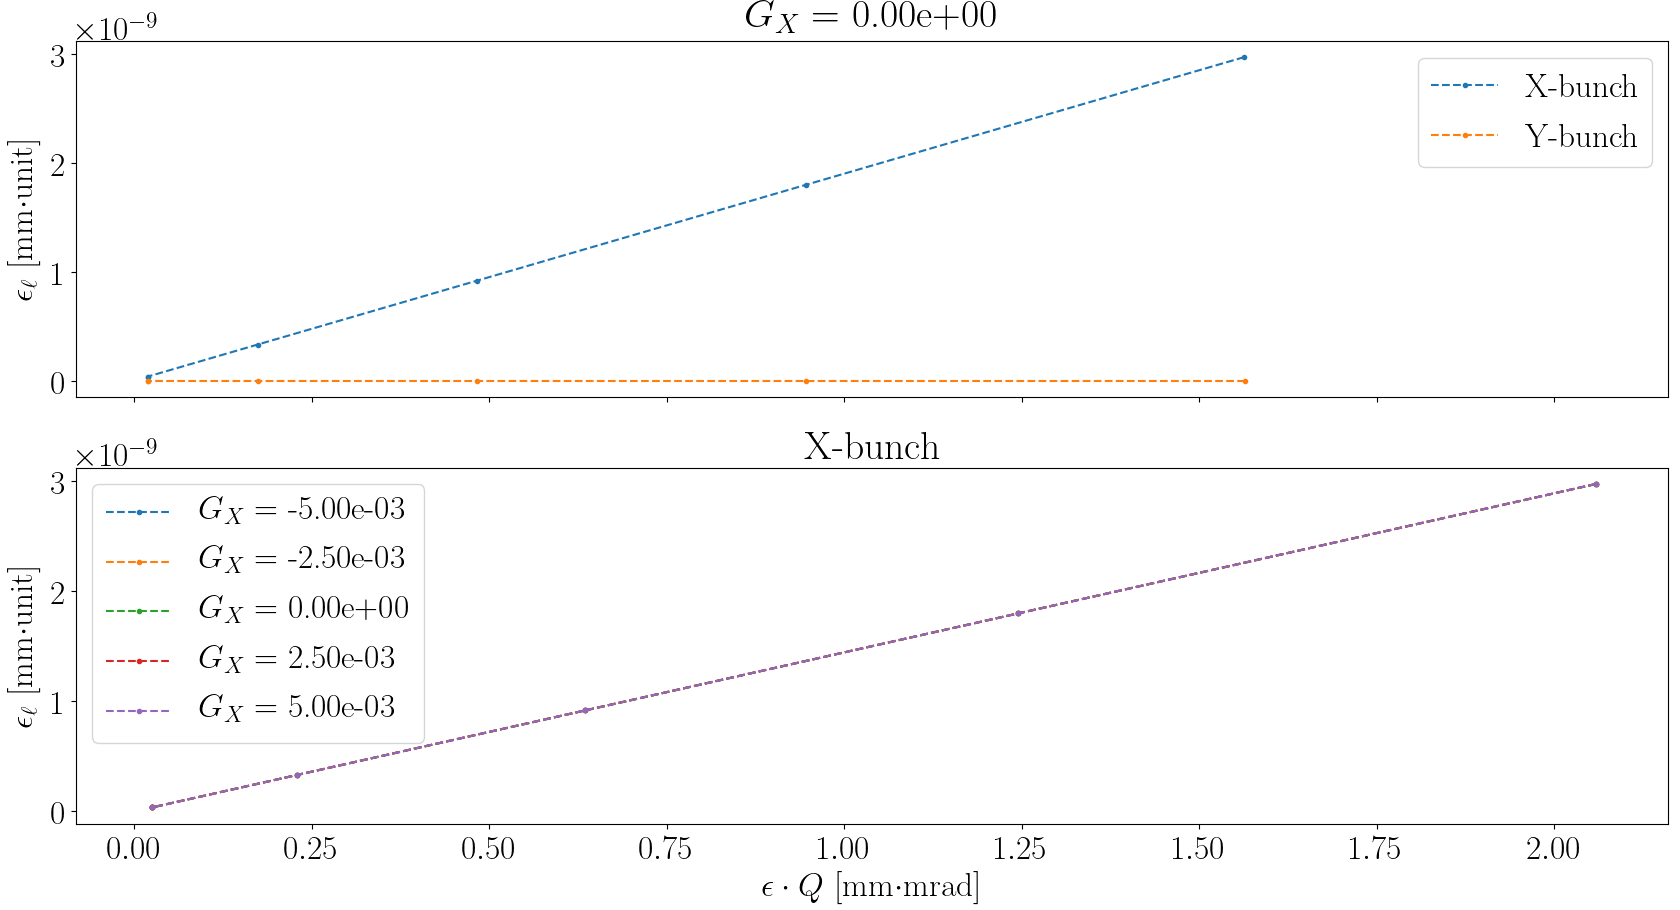
\includegraphics[height=.3\paperheight]{images/stune_traj_equ/part1/long_emitt_vs_trans_emitt_linear}
\caption{Linear transfer maps.}
\end{subfigure}
\caption{Longitudinal emittance as a function of
Q-normalized transverse emittance.\label{fig:long_emitt_vs_trans_emitt}}
\end{figure}

\paragraph{Conclusion:} formulation A of Statement 1 is false. 
